\documentclass[UTF8,zihao=-4,a4paper]{ctexart}
\usepackage{geometry}
\usepackage{graphicx}
\usepackage{booktabs}
\usepackage{tabularx}
\usepackage{array}
\usepackage{caption}
\usepackage{float}
\usepackage{hyperref}
\usepackage{setspace}
\usepackage{titlesec}
\usepackage{fancyhdr}

\geometry{left=2.8cm,right=2.8cm,top=2.5cm,bottom=2.5cm}
\setstretch{1.35}
\captionsetup[figure]{name=图,labelsep=quad,font=small}
\captionsetup[table]{name=表,labelsep=quad,font=small,position=top}
\titleformat{\section}{\heiti\zihao{4}}{\thesection}{0.8em}{}
\titleformat{\subsection}{\heiti\zihao{-4}}{\thesubsection}{0.8em}{}
\pagestyle{fancy}
\fancyhf{}
\fancyhead[C]{光权修复 AI 辅助空间决策工作流研究}
\fancyfoot[C]{\thepage}

\title{\heiti\zihao{2} 光权修复：面向旧街区采光修复的 AI 辅助空间决策工作流研究}
\author{}
\date{2026年6月3日}

\begin{document}
\maketitle

版本：v3，参考 Leey21/awesome-ai-research-writing 的“中转中-word”“表达润色（中文论文）”“逻辑检查”“Reviewer 视角审视”等写作流程整理。

日期：2026-06-03

\section{摘要}
旧街区更新中的采光不足，往往由高密度建筑、狭窄街巷和长期叠加的空间使用关系共同造成。传统建筑设计流程能够通过经验判断提出改造方向，但在早期阶段较难同时完成暗区定位、体块策略比较、指标复核和团队协作数据整理。本文以厦门灌口沿湖休闲片区为对象，构建一套面向旧街区采光修复的 AI 辅助空间决策工作流。该工作流将 CAD 标注、SketchUp/OBJ 白模、建筑编号、高度表和人工可改性判断转译为可计算数据，并通过“诊断、生成、复核”三个环节组织设计决策。

在方法上，算法 A 基于冬至日 8:00 至 16:00 的简化太阳路径和 2.5D 遮挡判断，生成采光热力图、平均采光小时和暗区比例。算法 B 在最小干预原则下生成保守型、均衡型和采光优先型三类候选策略。算法 C 对候选策略进行 post-simulation 复核，并将保守型方案重新转译为完整 SketchUp 场地模型，由组员补做算法前后的同视角人工光照分析。结果显示，在 6m 基准网格下，现状平均采光小时为 6.422h，暗区比例为 17.55\%；保守型 AI 方案将平均采光小时提高至 6.435h，暗区比例降低至 16.94\%，暗区改善比例约为 3.48\%，主要干预建筑为 C6 和 C33。进一步的 3m 网格敏感性测试显示，暗区比例与候选建筑排序会随采样尺度发生变化，说明当前简化模型更适合用于早期问题诊断与候选生成，而不宜替代专业日照软件。

本文的核心贡献不在于证明 AI 方案优于人工设计，而在于提出一种可复核的人机协同流程。AI 用于快速识别暗区、生成低干预候选方案和输出量化指标；设计团队则负责可改性判断、空间语言转译、人工光照复核和最终方案取舍。研究表明，在本科建筑设计团队的低成本工具条件下，AI 可以作为旧街区采光修复的早期决策助手，为方案讨论、论文图表和后续专业验证提供稳定的数据接口。

关键词：光权修复；旧街区更新；采光诊断；AI 辅助设计；空间决策；人机协同

\section{1 引言}
旧街区更新并不只是对建筑外观或空间功能的再设计，也涉及公共环境品质的修复。对于高密度街区而言，采光不足是最容易被居民感知、却又较难在早期设计中被精确处理的问题。狭窄街巷、高低错落的建筑体量和不规则的用地边界，会使局部公共空间长期处于阴影中。若仅依靠经验判断，设计团队可以发现一些明显问题，却难以快速比较不同体块调整策略的影响；若完全依赖专业日照软件，前期建模、参数设置和数据转译成本又较高，不一定适合本科团队在课程设计阶段反复迭代。

灌口沿湖休闲片区具有典型的旧街区空间特征。该片区建筑密度较高，街巷尺度紧凑，建筑高度和体块关系复杂。组员已经完成建筑编号、CAD 标注、SketchUp 白模和高度信息整理，为算法介入提供了基础。然而，任务书和官方材料并未明确规定所有建筑的可改与不可改属性。经组员确认，目前只有 C42 幼儿园被设定为不可动建筑，其余建筑可作为算法候选对象，但最终是否干预仍需结合结构、产权、功能和设计判断复核。

本研究在会议讨论后调整了问题表述。原先的设想是比较 AI 方案与人工方案的优劣，但这一比较容易引入过多不可控变量。人工方案往往包含课程目标、审美判断、功能组织、教师意见和表达策略，不能简单用采光指标判定优劣。本文因此将研究主线调整为：AI 如何嵌入旧街区采光修复流程，帮助设计团队完成暗区诊断、候选策略生成、指标验证和人工复核。换言之，本文关注的不是 AI 替代人工设计，而是 AI 如何成为空间决策过程中的辅助工具。

基于这一问题意识，本文提出“光权修复 AI 辅助空间决策工作流”。该工作流将建筑学调研资料转译为可计算数据，通过简化采光诊断识别暗区，通过最小干预策略生成候选方案，再通过 post-simulation、网格敏感性测试和人工同视角光照分析进行复核。研究希望证明，在低成本工具链下，AI 仍能为旧街区采光修复提供可讨论、可复核、可迭代的早期决策支持。

\section{2 文献综述}
城市形态与太阳可达性之间存在直接关系。Compagnon 对城市肌理中的太阳与自然光可达性进行了研究，指出城市尺度下的光环境评价应把建筑群体、街巷形态和开放空间作为整体考虑。Czachura 等对城市规划中的太阳性能指标进行了综述，强调太阳可达性指标适合在早期规划设计中提供反馈，但指标复杂度需要与设计阶段相匹配。对于本研究而言，平均采光小时、暗区比例和采样网格诊断属于低复杂度早期指标，适合用于问题定位和候选策略比较，但不能直接等同于专业日照审查结论。

太阳可达性不仅是评价指标，也可以反向塑造建筑体量。Curreli 等提出太阳能可以作为城市形态生成的重要依据，说明采光和太阳辐射并非后期附加条件，而是能够参与空间形态推导的环境因素。De Luca 等提出的反向太阳包络方法进一步表明，建筑体量可以在太阳可达性与法规框架约束下被生成或修正。这一思路与本文的光权修复目标相近，即通过局部体块退让、采光缝和屋顶平台释放街巷采光条件。

性能化设计研究为本文的算法流程提供了方法基础。Konis、Gamas 与 Kensek 提出的早期被动性能优化框架表明，建筑体量、朝向和局部形态可以通过模拟和优化方法获得反馈。EvoMass 相关研究进一步把体块类型探索与性能化优化结合起来，说明计算工具的价值并不只在于输出单一最优结果，也在于帮助设计者比较不同候选方案的性能差异。与这些研究相比，本文并不追求复杂的几何布尔或高精度环境模拟，而是强调数据结构稳定、团队可理解和结果可复核。

在人机协同方面，Thoring 等提出生成式 AI 应当增强设计师能力，而不是替代设计师。Rafsanjani 与 Nabizadeh 从 AEC 行业角度讨论以人为中心的 AI，强调 AI 系统需要保留人的判断、反馈和控制权。Jakubik 等在 AEC 平面图对象识别中采用 human-in-the-loop 机制，说明 AI 输出与人工复核结合可以提升系统可信度。本文据此将人工复核纳入方法本身：建筑可改性、模型同一性、空间转译和最终方案判断均由人工参与完成。

\section{3 研究对象与数据转译}
本文研究对象为厦门灌口沿湖休闲片区。项目数据主要包括 CAD/DXF 标注、SketchUp/OBJ 白模、建筑高度表、建筑变量表、策略对比数据和人工光照复核图。CAD/DXF 文件提供建筑编号、道路图层和高度标注；SketchUp/OBJ 白模提供建筑体块和场地空间关系；建筑变量表记录每栋建筑的边界、高度、底面积、体积、是否可动和是否保护等字段；人工光照图用于检查算法前后结果是否与同视角光照分析方向一致。

数据转译是本研究的关键步骤。算法并不是直接理解一张 CAD 图或一个 SketchUp 模型，而是通过统一编号、坐标和属性表识别建筑对象。只有当 CAD 标注、SU 组名和 CSV 表格中的建筑编号能够对应时，算法输出才具有可解释性和可复核性。对于重复编号的建筑组，本文根据组员说明将其作为同一建筑对象处理。对于 C42 幼儿园，因其被组员确认为不可动建筑，在算法中设置为不可干预对象。其余建筑在算法中作为候选对象，但这并不意味着它们在现实中一定可以直接改造。

\section{4 方法}
本文方法由三个算法环节和两个复核环节构成。算法 A 负责诊断，算法 B 负责生成候选策略，算法 C 负责验证与筛选。两个复核环节分别是网格敏感性测试和人工同视角光照复核。

算法 A 读取场地 OBJ 模型和建筑数据表，建立地面采样网格，并模拟厦门冬至日 8:00 至 16:00 的太阳路径。当前版本采用简化 2.5D 遮挡判断，将建筑近似为具有高度的体块，判断每个网格点在不同时间是否被周边建筑遮挡。算法输出包括平均采光小时、暗区比例、暗区坐标和采光热力图。该环节的目标是快速定位“哪里暗”和“哪些建筑可能影响暗区”，而不是取代专业日照软件。

算法 B 以算法 A 的暗区识别结果为输入，在最小干预原则下生成候选方案。本文设置三类策略。保守型 AI 优先降低干预体量和涉及建筑数量，均衡型 AI 在采光提升与改造代价之间折中，采光优先型 AI 更重视暗区改善并允许较大体量调整。评分逻辑综合考虑预估光照增益、干预体量、新增阴影惩罚和不可动建筑冲突。由于 C42 幼儿园被设为不可动建筑，算法不会对其进行削减。

算法 C 对候选策略进行 post-simulation，重新计算方案调整后的采光指标，并比较 baseline、保守型 AI、均衡型 AI 和采光优先型 AI 之间的差异。会议后，本文主问题已收敛到采光，因此可达性和安全规则只作为后续设计复核约束，不作为论文主指标。这样处理能够避免研究变量过多，使论文围绕采光修复形成清晰主线。

为了检查算法稳定性，本文补做 3m 网格敏感性测试。原始计算采用 6m 基准网格，3m 网格用于观察暗区比例和候选建筑排序是否随采样尺度变化。为了检查算法结果是否能回到建筑模型中被复核，本文将保守型方案转译为完整 SketchUp 场地模型。该模型保留原场地、道路、建筑位置和其他建筑，仅修改 C6 与 C33 的上部体量，并由组员补做算法前后同视角光照分析。

\section{5 结果}
在 6m 基准网格下，现状平均采光小时为 6.422h，暗区比例为 17.55\%。保守型 AI 方案后，平均采光小时提高至 6.435h，暗区比例降低至 16.94\%，暗区改善比例约为 3.48\%。该方案主要涉及 C6 和 C33 两栋建筑，简化干预体量为 28.125。均衡型和采光优先型在 post-simulation 后没有表现出明显优于保守型的采光结果，但干预体量更大。因此，在最小干预原则下，保守型 AI 被选为本文的推荐候选策略。

保守型方案的建筑学意义不应被理解为直接拆除。C6 原高度为 6.0m，算法建议高度为 4.5m，削减 1.5m。该变化可转译为屋顶边缘退台或上部轻量构筑物削减，设计上可形成屋顶平台和面向暗区的采光缝，同时保留底层街巷界面。C33 原高度为 9.0m，算法建议高度为 6.75m，削减 2.25m。该变化可转译为二层以上局部退台、转角采光缝和小型口袋灰空间。通过这种转译，算法输出从抽象体量变化转化为建筑学可讨论策略。

3m 网格敏感性测试显示，baseline 平均采光小时为 6.509h，暗区比例为 16.09\%。与 6m 网格相比，3m 网格下候选建筑排序发生变化，推荐对象转为 C28、C34、C38 和 C9，且 post-simulation 后暗区比例没有进一步下降。这一结果说明，当前简化算法对网格尺度存在敏感性，不能被表述为精确找到唯一最优建筑。更稳妥的表述是：该算法适用于早期问题定位和候选策略生成，最终方案仍需通过人工判断和专业光照工具复核。

人工同视角光照复核补强了论文证据链。算法后模型不是孤立建筑或空 OBJ，而是从原始完整场地 SKP 转换而来，保留了道路、场地边界、其他建筑和整体空间关系，只修改 C6 与 C33。组员基于算法前后两个完整 SKP 模型补做同视角光照分析。复核图显示，算法后模型能够被放回完整场地中检查，并与 AI 诊断方向进行对照。论文中应将该结果表述为方向性复核证据，而不应写成专业日照软件已经完全证明算法精确。

\section{6 讨论}
本文最重要的方法调整，是将研究从“AI 与人工方案谁更好”转向“AI 如何辅助空间决策”。这一转向使变量更加可控，也更符合建筑设计研究的逻辑。人工方案包含审美、功能、课程表达和教师反馈等多重因素，若直接与 AI 方案比较，容易把研究问题混杂化。将比较对象改为 baseline、保守型 AI、均衡型 AI 和采光优先型 AI 后，研究能够在同一套指标、同一套模型和同一套规则下讨论算法策略差异。

简化模型的价值在于低成本、可解释和易复核。当前工作流使用 Python、CSV、OBJ 和 SketchUp 模型，不依赖复杂商业插件。对于本科团队而言，这种方式降低了数据整理和协作门槛，也使每一步输出都能被组员检查。与此同时，简化模型的局限也很明确。2.5D 遮挡判断无法达到专业日照软件精度，网格尺度会影响结果，OBJ 白模的几何质量也会影响建筑识别。因此，论文必须保留“早期决策支持”的定位，而不是宣称系统已经完成专业日照审查。

最小干预原则使保守型方案具有较强的建筑学解释力。虽然保守型方案带来的指标提升幅度不大，但它涉及建筑少、干预体量小，更符合旧街区更新中的现实约束。C6 和 C33 的局部退台、屋顶平台和采光缝策略，能够在保持街巷结构的前提下释放局部采光条件。这类策略比大规模削减更容易进入课程设计讨论，也更符合有机更新和微更新的表达方式。

从证据链角度看，本文已经形成较完整的工作流。CAD/SU/OBJ 与建筑表构成数据底座，算法 A 提供暗区诊断，算法 B 提供候选策略，算法 C 提供 post-simulation，网格敏感性测试揭示模型局限，人工同视角光照分析提供外部复核，C6 和 C33 的设计转译则把算法输出转化为空间语言。这条链条能够支撑论文初稿，但正式提交前仍需补充图题、表题、图版排版和参考文献格式。

\section{7 结论}
本文以厦门灌口沿湖休闲片区为对象，构建了一个面向旧街区采光修复的 AI 辅助空间决策工作流。研究将 CAD 标注、SketchUp/OBJ 白模、建筑高度表和人工规则转译为可计算数据，并通过诊断、生成和复核三个环节完成暗区识别、候选策略生成和结果验证。

在 6m 基准网格下，保守型 AI 策略使暗区比例从 17.55\% 降至 16.94\%，平均采光小时从 6.422h 提升至 6.435h。虽然提升幅度有限，但该策略干预体量较小，主要涉及 C6 与 C33，适合转译为局部退台、屋顶平台和采光缝等建筑策略。3m 网格敏感性测试显示，当前简化模型对采样尺度存在敏感性，因此算法输出应被定位为候选决策支持，而不是唯一最优方案。

人工同视角光照复核进一步说明，AI 候选可以回到完整场地模型中被检查，并作为设计团队讨论和论文图表表达的依据。总体而言，本研究的价值在于建立了一套人机协同的光环境修复流程。AI 负责快速诊断与候选生成，人工负责可改性判断、设计转译和最终复核。该流程为旧街区更新中的采光问题提供了一种低成本、可复核、可扩展的研究路径。

1. Czachura, A., Kanters, J., Gentile, N., \& Wall, M. (2022). Solar Performance Metrics in Urban Planning: A Review and Taxonomy. Buildings, 12(4), 393. https://doi.org/10.3390/buildings12040393

2. Compagnon, R. (2004). Solar and daylight availability in the urban fabric. Energy and Buildings, 36(4), 321-328. https://doi.org/10.1016/j.enbuild.2004.01.009

3. Allegrini, J., Dorer, V., \& Carmeliet, J. (2015). Review of the impact of urban block form on thermal performance, solar access and ventilation. Renewable and Sustainable Energy Reviews, 38, 551-560. https://doi.org/10.1016/j.rser.2014.06.007

4. Curreli, A., Serra-Coch, G., Isalgue, A., Crespo, I., \& Coch, H. (2016). Solar Energy as a Form Giver for Future Cities. Energies, 9(7), 544. https://doi.org/10.3390/en9070544

5. Konis, K., Gamas, A., \& Kensek, K. (2016). Passive performance and building form: An optimization framework for early-stage design support. Solar Energy, 125, 161-179. https://doi.org/10.1016/j.solener.2015.12.020

6. Wang, L. et al. (2024). Optimization-based design exploration of building massing typologies: EvoMass and a typology-oriented computational design optimization method for early-stage performance-based building massing design. Frontiers of Architectural Research, 13(6), 1400-1422. https://doi.org/10.1016/j.foar.2024.06.001

7. Sadeghipour Roudsari, M., \& Pak, M. (2013). Ladybug: A Parametric Environmental Plugin for Grasshopper to Help Designers Create an Environmentally-Conscious Design. Proceedings of BS2013. https://www.ladybug.tools/publication.html

8. De Luca, F. et al. (2021). Reverse solar envelope method. A new building form-finding method that can take regulatory frameworks into account. Automation in Construction, 123, 103518. https://doi.org/10.1016/j.autcon.2020.103518

9. Thoring, K., Huettemann, S., \& Mueller, R. M. (2023). The Augmented Designer: A Research Agenda for Generative AI-enabled Design. Proceedings of the Design Society, 3, 3345-3354. https://doi.org/10.1017/pds.2023.335

10. Jakubik, J., Hemmer, P., Vössing, M., Blumenstiel, B., Bartos, A., \& Mohr, K. (2022). Designing a Human-in-the-Loop System for Object Detection in Floor Plans. Proceedings of the AAAI Conference on Artificial Intelligence, 36(11), 12524-12530. https://doi.org/10.1609/aaai.v36i11.21522

11. Rafsanjani, H. N., \& Nabizadeh, A. H. (2023). Towards human-centered artificial intelligence (AI) in architecture, engineering, and construction (AEC) industry. Computers in Human Behavior Reports, 11, 100319. https://doi.org/10.1016/j.chbr.2023.100319


\section{图表与表格}

\begin{figure}[H]
\centering
\includegraphics[width=0.88\textwidth]{figures/algorithm_heatmap.png}
\caption{现状采光热力图。该图展示 baseline 状态下场地冬至日简化采光诊断结果，用于定位整体暗区分布。}
\end{figure}

\begin{figure}[H]
\centering
\includegraphics[width=0.88\textwidth]{figures/strategy_comparison_chart.png}
\caption{三类 AI 策略指标对比。该图比较 baseline、保守型、均衡型与采光优先型策略的核心指标。}
\end{figure}

\begin{figure}[H]
\centering
\includegraphics[width=0.88\textwidth]{figures/grid_sensitivity_chart_partial.png}
\caption{网格敏感性测试结果。该图比较 6m 与 3m 网格下采光诊断与候选结果的变化。}
\end{figure}

\begin{figure}[H]
\centering
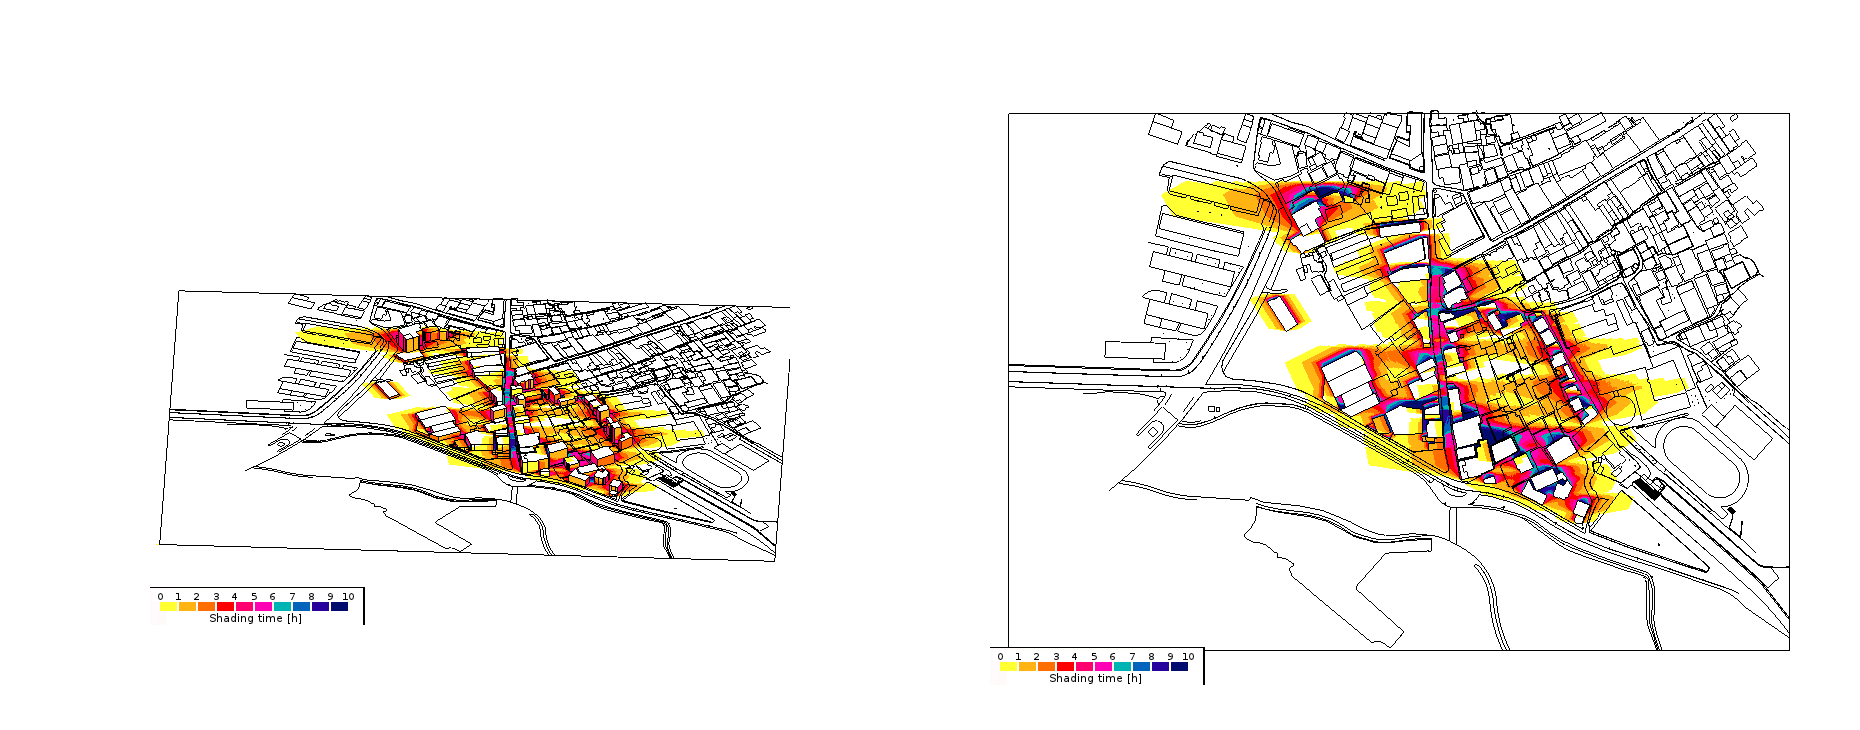
\includegraphics[width=0.96\textwidth]{figures/manual_validation_before_after.png}
\caption{算法前后同视角人工光照复核。算法后模型保留完整场地，仅调整 C6 与 C33，用于方向性复核。}
\end{figure}

\begin{table}[H]
\centering
\caption{baseline 与三类 AI 策略对比指标}
\small
\begin{tabular}{p{0.13\textwidth}p{0.13\textwidth}p{0.13\textwidth}p{0.13\textwidth}p{0.13\textwidth}p{0.13\textwidth}}
\toprule
方案类型 & 平均采光小时 & 暗区比例 & 干预体量 & 涉及建筑 & 保护冲突 \\
\midrule
baseline & 6.422 & 17.55\textbackslash{}\% & 0.0 &  & 0 \\
AI\_conservative & 6.435 & 16.94\textbackslash{}\% & 28.125 & C33;C6 & 0 \\
AI\_balanced & 6.435 & 16.94\textbackslash{}\% & 45.0 & C33;C6 & 0 \\
AI\_light\_first & 6.435 & 16.94\textbackslash{}\% & 46.095 & C33;C6;C9 & 0 \\
\bottomrule
\end{tabular}
\end{table}

\begin{table}[H]
\centering
\caption{6m 与 3m 网格敏感性测试结果}
\small
\begin{tabular}{p{0.13\textwidth}p{0.13\textwidth}p{0.13\textwidth}p{0.13\textwidth}p{0.13\textwidth}p{0.13\textwidth}p{0.13\textwidth}}
\toprule
网格尺寸 & 现状平均采光小时 & 现状暗区比例 & 方案后平均采光小时 & 方案后暗区比例 & 改善比例 & 候选建筑 \\
\midrule
 & 6.422 & 17.55\textbackslash{}\% & 6.435 & 16.94\textbackslash{}\% & 3.48\textbackslash{}\% & C33;C6 \\
 & 6.509 & 16.09\textbackslash{}\% & 6.509 & 16.09\textbackslash{}\% & 0.00\textbackslash{}\% & C28;C34;C38;C9 \\
\bottomrule
\end{tabular}
\end{table}

\begin{table}[H]
\centering
\caption{保守型方案中 C6、C33 的高度变化与设计转译}
\small
\begin{tabular}{p{0.12\textwidth}p{0.12\textwidth}p{0.14\textwidth}p{0.14\textwidth}p{0.34\textwidth}}
\toprule
建筑编号 & 原高度/m & 算法后高度/m & 削减高度/m & 设计转译 \\
\midrule
C6 & 6.0 & 4.5 & 1.5 & 屋顶边缘退台、屋顶平台、采光缝。\\
C33 & 9.0 & 6.75 & 2.25 & 二层以上局部退台、转角采光缝、口袋灰空间。\\
\bottomrule
\end{tabular}
\end{table}

\section{参考文献}
\begin{enumerate}
\item CZACHURA A, KANTERS J, GENTILE N, 等. Solar performance metrics in urban planning: a review and taxonomy[J]. Buildings, 2022, 12(4): 393. DOI: 10.3390/buildings12040393.
\item COMPAGNON R. Solar and daylight availability in the urban fabric[J]. Energy and Buildings, 2004, 36(4): 321-328. DOI: 10.1016/j.enbuild.2004.01.009.
\item ALLEGRINI J, DORER V, CARMELIET J. Review of the impact of urban block form on thermal performance, solar access and ventilation[J]. Renewable and Sustainable Energy Reviews, 2015, 38: 551-560. DOI: 10.1016/j.rser.2014.06.007.
\item CURRELI A, SERRA-COCH G, ISALGUE A, 等. Solar energy as a form giver for future cities[J]. Energies, 2016, 9(7): 544. DOI: 10.3390/en9070544.
\item KONIS K, GAMAS A, KENSEK K. Passive performance and building form: an optimization framework for early-stage design support[J]. Solar Energy, 2016, 125: 161-179. DOI: 10.1016/j.solener.2015.12.020.
\item WANG L, 等. Optimization-based design exploration of building massing typologies: EvoMass and a typology-oriented computational design optimization method for early-stage performance-based building massing design[J]. Frontiers of Architectural Research, 2024, 13(6): 1400-1422. DOI: 10.1016/j.foar.2024.06.001.
\item SADEGHIPOUR ROUDSARI M, PAK M. Ladybug: a parametric environmental plugin for Grasshopper to help designers create an environmentally-conscious design[C]//Proceedings of BS2013. 2013.
\item DE LUCA F, 等. Reverse solar envelope method: a new building form-finding method that can take regulatory frameworks into account[J]. Automation in Construction, 2021, 123: 103518. DOI: 10.1016/j.autcon.2020.103518.
\item THORING K, HUETTEMANN S, MUELLER R M. The augmented designer: a research agenda for generative AI-enabled design[C]//Proceedings of the Design Society. 2023, 3: 3345-3354. DOI: 10.1017/pds.2023.335.
\item JAKUBIK J, HEMMER P, VÖSSING M, 等. Designing a human-in-the-loop system for object detection in floor plans[J]. Proceedings of the AAAI Conference on Artificial Intelligence, 2022, 36(11): 12524-12530. DOI: 10.1609/aaai.v36i11.21522.
\item RAFSANJANI H N, NABIZADEH A H. Towards human-centered artificial intelligence (AI) in architecture, engineering, and construction (AEC) industry[J]. Computers in Human Behavior Reports, 2023, 11: 100319. DOI: 10.1016/j.chbr.2023.100319.
\end{enumerate}

\end{document}
